\chapter{IF toolset}
\label{sec:if}

\section{Instructions}

\begin{description}
\item[\textcolor{green}{Author}]  Huu Nghia \textsc{Nguyen} (Instiut T\'el\'ecom-SudParis)
\item[\textcolor{blue}{Assessor 1}] First assessor of the approaches \todo{Name - Company}
\item[\textcolor{magenta}{Assessor 2}] Second assessor of the approaches \todo{Name - Company}
\end{description}

In the sequel, main text is under the responsibilities of the author.

\begin{author_comment}
Author can add comments using this format at any place.
\end{author_comment}

\begin{assessor1}
First assessor can add comments using this format at any place.
\end{assessor1}

\begin{assessor2}
Second assessor can add comments using this format at any place.
\end{assessor2}

When a note is required, please follow this list (inspired from Technology Readiness Level, see \url{http://en.wikipedia.org/wiki/Technology\_readiness\_level}) :

\begin{description}
\item[0] not recommended / rejected / no integration possible or valuable / not adapted for this topic / not available for this topic
\item[1] weakly recommended / adapted after major improvements / weakly rejected / concept of integration roughly defined / adapted after major improvements / available after major developments
\item[2] recommended / adapted (with light improvements if necessary)  weakly accepted / integration prototyped or defined in details / adapted after small improvements / available after small developments or tests
\item[3] highly recommended / well adapted / strongly accepted / integration done and tested / well adapted to the purpose / available and suitable for the purpose All the notes can be commented under each table.
\item[*] difficult to evaluate with a note (please add a comment under the table)
\end{description}


All the notes can be commented under each table.

This section defines the criteria for the means and tools dedicated to verification and validation activities, in the WP4 workpackage. 

Criteria of this section are defined according \citep{D4.1}.

\section{Presentation}

This section gives a quick presentation of the approach and the tool.

\begin{description}
\item[Name]  IF toolset (IF)
\item[Web site]  \url{http://www-if.imag.fr}
\item[Licence]  This software may be freely used, copied and redistributed without fee for non-commerical purpose
\end{description}

\paragraph{Abstract}  
%The IF toolset provides an environment for verification of Intermediate Language  (IF) specifications. IF is an intermediate representation dedicated for timed asynchronous communicating systems. It represent a system by a set of parallel processes communicating asynchronously through a set of buffers. An IF process is described as a timed automaton extended with data. It has an unique identifier, a set of control states, a private queue of pending messages (received and not yet consumed), and local data such as discrete variables and clocks. A transition between two states can be triggered either by (timed) guards or by an input message. The effect actions of a transition may include sending output messages, setting/resetting clocks, assignment of variable values, and creation/destruction of processes.


The IF toolset which is an environment for modelling and validation of heterogeneous real-time systems. The toolset is built upon a rich formalism, the Intermediate Language  (IF) notation, allowing structured automata-based system representations. Moreover, the IF notation is expressive enough to support real-time primitives and extensions of high-level modelling languages such as SDL and UML/SysML by means of structure preserving mappings. The core part of the IF toolset consists of a syntactic transformation component and an open exploration platform. The syntactic transformation component provides language level access to IF descriptions and has been used to implement static analysis and optimisation techniques. The exploration platform gives access to the graph of possible executions. It has been connected to different state-of-the-art model-checking and test-case generation tools.

\paragraph{Publications} Please refer to \url{http://www-if.imag.fr/papers.html}


\section{Common criteria on secondary means and tools}
\label{common}
This section discusses the common criteria of the means and tools according to the project requirements on tools and the results of T7.1.

\subsection{Project and WP2 requirements}

The objectives of this list of criteria is to check if the proposed means and tools meet the main criteria of the project: open-source approaches, usability, modularity, coverage of the objectives,...

According WP2 requirements, give a note for characteristics of the use of the tool (from 0 to 3) :

\begin{tabular}{|l | c | c | c | c|}
\hline
& \textcolor{green}{Author} & \textcolor{blue}{Assessor 1} & \textcolor{magenta}{Assessor 2} & Total \\
\hline 
Open Source (D2.6-02-074) & 2* & & &  \\
\hline 
Portability to operating systems (D2.6-02-075) & 3** & & &  \\
\hline
Cooperation of tools (D2.6-02-076) & 2 & & &  \\
\hline
Robustness (D2.6-02-078) & 2 & & & \\
\hline
Modularity (D2.6-02-078.1) & 2 & & & \\
\hline
Documentation management (D2.6-02-078.02) & 0 & & & \\
\hline
Distributed software development (D2.6-02-078.03)  & 0 & & & \\
\hline
Simultaneous multi-users (D2.6-02-078.04)   & 1*** & & & \\
\hline
Issue tracking (D2.6-02-078.05) & 0 & & & \\
\hline
Differences between models (D2.6-02-078.06) & 0 & & & \\
\hline
Version management (D2.6-02-078.07) & 0 & & & \\
\hline
Concurrent version development (D2.6-02-078.08) & 0 & & & \\
\hline
Model-based version control (D2.6-02-078.09) & 0 & & & \\
\hline
Role traceability (D2.6-02-078.10) & 0 & & & \\
\hline
Safety version traceability (D2.6-02-078.11) & 0 & & & \\
\hline
Model traceability (D2.6-02-079) & 0 & & & \\
\hline
Tool chain integration & 2 & & & \\
\hline
Scalability & 2 & & & \\
\hline
User Friendliness & 2 & & & \\
\hline
\end{tabular}


\begin{author_comment}

	* The source code can be retrieved from its API document \url{http://www-if.imag.fr/apis.html}
	
	** Currently, it can run on Mac OSX 10.6 and above, Linux, Windows (thanks to Cygwin), and Solaris 2.8
	
	
	*** Multi simulators can connect simultaneously to the tool
	
\end{author_comment}

\subsection{Qualification}

This section discusses how the tool can be classified according EN50128 requirements (D2.6-02-085). Some qualification shall be mandatory  if the tool is involved to design a SIL4 software.


\begin{tabular}{|l | c | c | c | c|}
\hline
& \textcolor{green}{Author} & \textcolor{blue}{Assessor 1} & \textcolor{magenta}{Assessor 2} & Total \\
\hline 
Tool manual (D.2.6-01-42.02) & 3 & & &  \\
\hline
Proof of correctness (D.2.6-01-42.03)   & 2 & & & \\
\hline
Existing industrial  usage  & 1 & & & \\
\hline
Model verification & 3 & & & \\
\hline
Test generation & 3 & & & \\
\hline
Simulation, execution, debugging & 2 & & & \\
\hline
Formal proof & 1 & & & \\
\hline
\end{tabular}

\begin{author_comment}
	
%	* e.g., Ariane 5 Flight program (\url{http://www-verimag.imag.fr/PEOPLE/mounier/Papers/Bozga-Lesens-Mounier-01.pdf})
	
\end{author_comment}

Which level of tool qualification has been reached or will be reached within the next year ?

Score :
\begin{description}
\item[3] already qualified for this level
\item[2] qualification possible to this level, but some elements shall be provided
\item[0] qualification not recommended for this level
\end{description}


\begin{tabular}{|l | c | c | c | c|}
\hline
& \textcolor{green}{Author} & \textcolor{blue}{Assessor 1} & \textcolor{magenta}{Assessor 2} & Total \\
\hline 
class T1 & 3 & & &  \\
\hline
class T2   & 3 & & & \\
\hline
class T3  & 0 & & & \\
\hline
\end{tabular}

%\begin{author_comment}
	
%	* Generation of test cases
%\end{author_comment}

\paragraph{Other elements for tool certification}


\subsection{Complementarity with primary toolchain}

The objectives of this list of criteria is to check if the proposed means and tools can be easily integrated to the primary toolchain.

\subsubsection{Language}


According to the decisions and the propositions of T7.1, how the mean and approach can be adapted to or can complete the chosen language and methods:

\begin{tabular}{|l | c | c | c | c|}
\hline
& \textcolor{green}{Author} & \textcolor{blue}{Assessor 1} & \textcolor{magenta}{Assessor 2} & Total \\
\hline 
SysML  & 2 & & & \\
\hline
Scade method & 0 & & & \\
\hline
EFS language & 0 & & & \\
\hline
B Method & 0 & & & \\
\hline
C language & 3 & & & \\
\hline
\end{tabular}

\paragraph{SysML}
How the means or tools can complete SysML ?

\begin{author_comment}
	\begin{itemize}
		\item Transformation from SysML, e.g., by using IFx-OMEGA (\url{http://www.irit.fr/ifx/})
	\end{itemize}
\end{author_comment}

\paragraph{Scade, EFS, Classical B}
How the means or tools can complete the current proposals for formal modeling language ?

\paragraph{C language}
How the means or tools can complete or be adapted to SIL4 software in C language ?

\begin{author_comment}
	\begin{itemize}
		\item An IF description is translated into a C program which is then compiled and executed to get outputs
	\end{itemize}
\end{author_comment}

\subsubsection{Tools and platforms}

According to the decisions and the propositions of T7.1, how the mean and approach can be integrated to or can complete the chosen tools and platforms:

\begin{tabular}{|l | c | c | c | c|}
\hline
& \textcolor{green}{Author} & \textcolor{blue}{Assessor 1} & \textcolor{magenta}{Assessor 2} & Total \\
\hline 
Eclipse & 1 & & &  \\
\hline
Papyrus  & 3 & & & \\
\hline
Scade & 0 & & & \\
\hline
EFS tools & 0 & & & \\
\hline
B tools & 0 & & & \\
\hline
\end{tabular}


\paragraph{Eclipse}
How the means or tools can be integrated to the Eclipse platform ?

\begin{author_comment}
		We can use any text editor in Eclipse to create/modify IF description. Eclipse can compile and run this description by "External Tools" command that will call IF toolset.
\end{author_comment}

\paragraph{Papyrus}
How the means or tools can complete  Papyrus ?

\begin{author_comment}
	The  output of Papyrus is an input of the tool. 
\end{author_comment}


\paragraph{Scade, EFS, Classical B}
How the means or tools can complete the current proposals for formal modeling tools ?





\section{VnV Activities}

The VnV activities are described in details in the verification and Validation Plan  \citep{D4.1}.

\begin{figure}[htb]
  \centering
  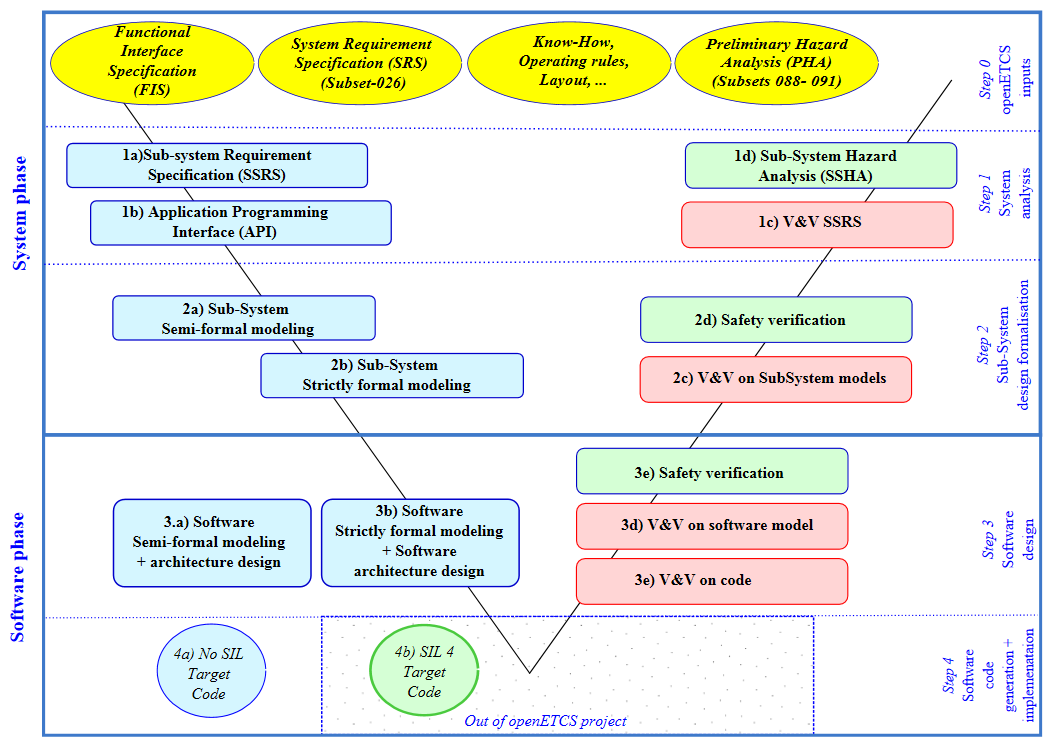
\includegraphics[width=.9\textwidth]{images/ProcessOpenETCS-BeM.png}
  \caption{openETCS Process (rough view)}
  \label{fig:openETCSProcess}
\end{figure}

According figure \ref{fig:openETCSProcess}, for which activities is the mean or tool suitable (see also \citep{D4.1} section 5.1.2 for more details)\footnote{DAS2V : Design Artifact Subject to Verification and Validation, see \citep{D4.1}} ?


\begin{tabular}{|l | c | c | c | c|}
\hline
& \textcolor{green}{Author} & \textcolor{blue}{Assessor 1} & \textcolor{magenta}{Assessor 2} & Total \\
\hline 
1c SSRS Verification & 3 & & &  \\
\hline
1c SSRS Validation & 3 & & &  \\
\hline
2c SFM Verification & 2 & & &  \\
\hline
2c SFM Validation & 2 & & &  \\
\hline
3d SW-SFM Verification & 2 & & &  \\
\hline
3d SW-SFM Validation & 2 & & &  \\
\hline
3d SW-FFM Verification & 3 & & &  \\
\hline
3d SW-FFM Validation & 3 & & &  \\
\hline
3e Code Verification & 0 & & &  \\
\hline
3e Code Validation & 0 & & &  \\
\hline
DAS2V Verification & 3 & & &  \\
\hline
DAS2V Validation & 3 & & &  \\
\hline
Automatic model transformation verification & 0 & & &  \\
\hline
Automatic code generation verification & 0 & & &  \\
\hline
\end{tabular}

\begin{author_comment}
	Assuming that SW-SFM means Software Semi Formal Model and SW-FFM means Software Fully Formal Model
\end{author_comment}

\section{Properties}

Which kind of properties or elements are verified or validated by the mean or tool (see also \citep{D4.1} section 4)  ?



\begin{tabular}{|l | c | c | c | c|}
\hline
& \textcolor{green}{Author} & \textcolor{blue}{Assessor 1} & \textcolor{magenta}{Assessor 2} & Total \\
\hline 
Functionalities of the system and sub-system & 3 & & &  \\
\hline
System and sub-system architecture & 0 & & &  \\
\hline
External and internal interfaces of sub-system & 1 & & &  \\
\hline
Software components & 3 & & &  \\
\hline
Performance constraints & 2* & & &  \\
\hline
Safety objectives & 3 & & &  \\
\hline
Functional properties & 3 & & &  \\
\hline
Safety properties & 3 & & &  \\
\hline
\end{tabular}

\begin{author_comment}
	* e.g., execution time
\end{author_comment}


\section{Verification methods and tools}

Which kind of methods is proposed (see also \citep{D4.1} section 5.3) ?



\begin{tabular}{|l | c | c | c | c|}
\hline
& \textcolor{green}{Author} & \textcolor{blue}{Assessor 1} & \textcolor{magenta}{Assessor 2} & Total \\
\hline 
Reviews & 0 & & &  \\
\hline
Inspections & 0 & & &  \\
\hline
Software Architecture Analysis Method & 0 & & &  \\
\hline
Architecture Tradeoff Analysis Method & 0 & & &  \\
\hline
Model-Based System Integration Testing & 0 & & &  \\
\hline
Model-Based Testing of Generated High-Level Code & 0 & & &  \\
\hline
Abstract Interpretation & 0 & & &  \\
\hline
Deductive Verification & 0 & & &  \\
\hline
Model Checking & 3 & & &  \\
\hline
Correct by Construction Formal Methods & 0 & & &  \\
\hline
Verification with Formal Methods & 3 & & &  \\
\hline
Simulation-based & 3 & & &  \\
\hline
\end{tabular}

\section{Validation means and tools}

The following list of criteria focuses on means and tools to support validation activities, according WP2  requirements :

\begin{tabular}{|l | c | c | c | c|}
\hline
& \textcolor{green}{Author} & \textcolor{blue}{Assessor 1} & \textcolor{magenta}{Assessor 2} & Total \\
\hline 
Simulation-based & 3 & & &  \\
\hline
Step-by-step simulation (D2.6-01-036) & 3 & & &  \\
\hline
Environment emulation (D2.6-01-037 and D2.6-02-080) & 2 & & &  \\
\hline
Time-based test case (D2.6-02-081) & 2 & & &  \\
\hline
Test cases writing (D2.6-01-038) & 1* & & &  \\
\hline
Test cases execution (D2.6-01-038) & 1* & & &  \\
\hline
Test cases storage (D2.6-01-038) & 1* & & &  \\
\hline
Version management of test cases (D2.6-02-082) & 0 & & &  \\
\hline
Test generation from independant test model (D2.6-02-083) & 2 & & &  \\
\hline
Test sequences writing (D2.6-02-084) & 1* & & &  \\
\hline
Test sequences execution (D2.6-02-084) & 1* & & &  \\
\hline
Test sequences storage (D2.6-02-084) & 1* & & &  \\
\hline
\end{tabular}

\begin{author_comment}
 * By encoding them into IF observers

\end{author_comment}

\section{VnV artifacts}


Concerning the artifacts used or produced by the mean or tool, please to detail:

\paragraph{Input}
    Which is the list of the input artifacts for the mean or tools ?
    
\begin{author_comment}

	A text file, in IF syntax, containing:
\begin{itemize}
	\item models of components of systems in timed automaton extended with data
	\item optionally, observers representing properties to be verified
\end{itemize}

The other input can be in format of  SDL, UML or SysML which will be translated automatically into IF thanks to existing modules in IF toolset.

\end{author_comment}
    
    
\paragraph{Output}
    Which is the list of the output artifacts for the mean or tools ?

\begin{author_comment}
	Depending on usage, the outputs may be:
	\begin{itemize}
		\item Results from model verification with error traces / states
		\item Test cases
		\item Visualisation of system execution
	\end{itemize}
\end{author_comment}
    
\paragraph{Syntax}
    Which are the reference documents which give a description of the artifacts syntax  ?
    
\begin{author_comment}
	\begin{itemize}
		\item \url{http://www-if.imag.fr/tutorials/syntax.ps.gz}
		\item \url{http://www-if.imag.fr/tutorials.html}
	\end{itemize}
\end{author_comment}
    
    
\paragraph{Semantic}
    Which are the reference documents which give a description of the artifacts semantic  ?

\begin{author_comment}
	\begin{itemize}
		\item \url{http://www-if.imag.fr/tutorials/semantics.ps.gz}
		\item \url{http://www-if.imag.fr/tutorials.html}
	\end{itemize}
\end{author_comment}



\paragraph{Integration}
    How these artifacts can be integrated with the elements of the toolchain (language, mangement,...) ?

\begin{author_comment}
	See above.
\end{author_comment}

\section{Detailled Criterias for VnV}

Please  fill only the section concerning the proposed mean or tool, other section can be skipped (see issue \url{https://github.com/openETCS/toolchain/issues/180} for details and discussions)



\subsection{System Modelling simulation}	

\begin{tabular}{|l | c | c | c | c|}
\hline
& \textcolor{green}{Author} & \textcolor{blue}{Assessor 1} & \textcolor{magenta}{Assessor 2} & Total \\
\hline 
User Scenario Modelling & 3 & & &  \\
\hline
Test Case Modelling & 2 & & &  \\
\hline
Test Sequence Modelling & 2 & & &  \\
\hline
\end{tabular}
	
\subsection{System Model Verification}	


\begin{tabular}{|l | c | c | c | c|}
\hline
& \textcolor{green}{Author} & \textcolor{blue}{Assessor 1} & \textcolor{magenta}{Assessor 2} & Total \\
\hline 
Input/ Output checking & 3 & & &  \\
\hline
System Behavior Simulation (Mathematical) & 3 & & &  \\
\hline
System Behavior Simulation (Animated) & 2 & & &  \\
\hline
\end{tabular}


\subsection{Software Model Verification	}


\begin{tabular}{|l | c | c | c | c|}
\hline
& \textcolor{green}{Author} & \textcolor{blue}{Assessor 1} & \textcolor{magenta}{Assessor 2} & Total \\
\hline 
Static Model Verification & 3 & & &  \\
\hline
Property Proofing & 2* & & &  \\
\hline
Dynamic Testing & 0 & & &  \\
\hline
Automatic Test Generation & 3** & & &  \\
\hline
Input/ Output checking & 3 & & &  \\
\hline
Software Behaviour Simulation (Mathematical) & 3 & & &  \\
\hline
Software Behaviour Simulation (Animated) & 2 & & &  \\
\hline
\end{tabular}


\begin{author_comment}

	* by mean of model-checking, i.e., give a counter example or exhaustive verification

	** with the supports of TestGen-IF or TGV test generator
	
\end{author_comment}

\subsection{Source Code}


\begin{tabular}{|l | c | c | c | c|}
\hline
& \textcolor{green}{Author} & \textcolor{blue}{Assessor 1} & \textcolor{magenta}{Assessor 2} & Total \\
\hline 
Traceability to Model & & & &  \\
\hline
\end{tabular}


\subsection{Code Verification	}


\begin{tabular}{|l | c | c | c | c|}
\hline
& \textcolor{green}{Author} & \textcolor{blue}{Assessor 1} & \textcolor{magenta}{Assessor 2} & Total \\
\hline 
Formal Proof & & & &  \\
\hline
Programming by contract & & & &  \\
\hline
Static Analysis & & & &  \\
\hline
Dynamic Analysis & & & &  \\
\hline
Dynamic Testing & & & &  \\
\hline
Automatic Test Generation & & & &  \\
\hline
Performance Testing & & & &  \\
\hline
Interface Testing & & & &  \\
\hline
\end{tabular}

	
\subsection{Validation System/Software/Code/ Validation	}


\begin{tabular}{|l | c | c | c | c|}
\hline
& \textcolor{green}{Author} & \textcolor{blue}{Assessor 1} & \textcolor{magenta}{Assessor 2} & Total \\
\hline 
Test Coverage & & & &  \\
\hline
Use Case Validation of Model & & & &  \\
\hline
Functional or Black-box Testing & & & &  \\
\hline
User Scenario Testing & & & &  \\
\hline
Traceability & & & &  \\
\hline
Schedulability Analyzer / UseCase Check all & & & &  \\
\hline
Schedulability Analyzer / UseCase Check single mode & & & &  \\
\hline

\end{tabular}



\section{Other comments}



\begin{comment}
This section is available for the author or the assessors to  complete the description and criteria.
\end{comment}



